\documentclass[english]{tktltiki2}

% --- General packages ---

\usepackage[utf8]{inputenc}
\usepackage[T1]{fontenc}
\usepackage{lmodern}
\usepackage{microtype}
%\usepackage[table,xcdraw]{xcolor}    % loads also »colortbl«
\usepackage{listings}
\usepackage{tabularx}
%\usepackage{minted}
%\usepackage{tcolorbox}
%\usepackage{etoolbox}
%\BeforeBeginEnvironment{minted}{\begin{tcolorbox}}%
%\AfterEndEnvironment{minted}{\end{tcolorbox}}%

\usepackage{amsfonts,amsmath,amssymb,amsthm,booktabs,enumitem,graphicx}
\usepackage{tocloft}
%\usepackage{relsize}
\usepackage[pdftex,hidelinks]{hyperref}
\usepackage[title]{appendix}
%\usepackage{tabularx}
%\usepackage[table]{xcolor}    % loads also »colortbl«
%\usepackage{float}

%\listfiles

\linespread{1.3}

\setlength{\intextsep}{18pt plus 2.0pt minus 2.0pt}

\lstset{%
  language=[LaTeX]TeX,
  basicstyle=\ttfamily,
  breaklines=true,
  columns=fullflexible,
}

%\setlength{\arrayrulewidth}{0.6pt}

% Automatically set the PDF metadata fields
\makeatletter
\AtBeginDocument{\hypersetup{pdftitle = {\@title}, pdfauthor = {\@author}}}
\makeatother

% --- Language-related settings ---
%
% these should be modified according to your language

% babelbib for non-english bibliography using bibtex
\usepackage[fixlanguage]{babelbib}
\selectbiblanguage{english}

% add bibliography to the table of contents
\usepackage[nottoc]{tocbibind}
% tocbibind renames the bibliography, use the following to change it back

\declarebtxcommands{english}{%
    \def\btxurldatecomment#1{ [#1]}%
}

% --- tktltiki2 options ---
%
% The following commands define the information used to generate title and
% abstract pages. The following entries should be always specified:

\title{Mining a Bird Observatory Dataset}
\author{Mikko Koho}
\date{\today}
\level{Technical report}

\abstract{
}

\keywords{}
%\classification{
%\textbf{} \\
%\textit{} \\
%\\
%}
% classification according to ACM Computing Classification System (http://www.acm.org/about/class/)
                  % This is probably mostly relevant for computer scientists

% If the automatic page number counting is not working as desired in your case,
% uncomment the following to manually set the number of pages displayed in the abstract page:
%



\begin{document}
    
% --- Front matter ---

\frontmatter      % roman page numbering for front matter

\maketitle        % title page

\makeabstract     % abstract page

\tableofcontents  % table of contents

% --- Main matter ---

\mainmatter       % clear page, start arabic page numbering


%%%%%%%%%%%%%%%%%%%
\section{Introduction}
%%%%%%%%%%%%%%%%%%%

This technical report examines the use of data mining techniques~\cite{tan2006introduction} to find interesting patterns from a bird observatory dataset.

Bird species names are written written with finnish, english and scientific names, to be accessible to different audiences. The format used is <finnish name, \emph{scientific name}, english name>.


%%%%%%%%%%%%%%%%%%%
\section{Related work}
%%%%%%%%%%%%%%%%%%%


%%%%%%%%%%%%%%%%%%%
\section{Dataset}
%%%%%%%%%%%%%%%%%%%

Hanko Bird Observatory, \emph{Halias}, is located at the southernmost tip of Finland in Hanko, Finland. Halias has been gathering bird observation data from 1979 onward and it has been used intensively in research~\cite{HangonJulkaisut}. However data mining or machine learning methods have been never applied to it, so these methods could perhaps uncover some interesting patterns in the data.

Gathering the data at Halias is highly standardized and main focus is on counting the daily migration of each bird species. Manning the station is based on volunteers, which causes some gaps in the data when no observers are present.
The dataset is not publicly available, but is available for research projects at request.

The data in original digital format consists of two Excel files, containing half a million rows of distinct daily counts per species for local and migrating birds from 1979 to 2009. Some rows contain a \emph{taxon} (plural \emph{taxa}) that is higher than species-level, for example a genus or a species pair.

However, in this case study we will be using a linked data publication made from the original dataset. The dataset has been transformed~\cite{koho-hyvonen-orni-2014, koho2015gradu} to RDF data model and linked with weather data from nearby weather station in Hanko, Russarö and a bird taxon ontology.
The linked dataset is structured using the RDF Data Cube Vocabulary~\cite{w3crdfdatacube}, containing distinct data cubes for both daily bird observations and daily weather observations. An example of the bird observation data in this format is given in figure \ref{fig: havaintograafi}.

The used bird taxon ontology~\cite{koho2015gradu} contains finnish conservation statuses for endangered species, a coarse measure of commonness at Halias and characteristics of many finnish species, such as size, beak color and plumage coloring. The taxon ontology is open and available\footnote{\url{http://www.ldf.fi/dataset/halias/rdf/halias_taxon_ontology.zip}}.

\begin{figure}[htb]
\centering
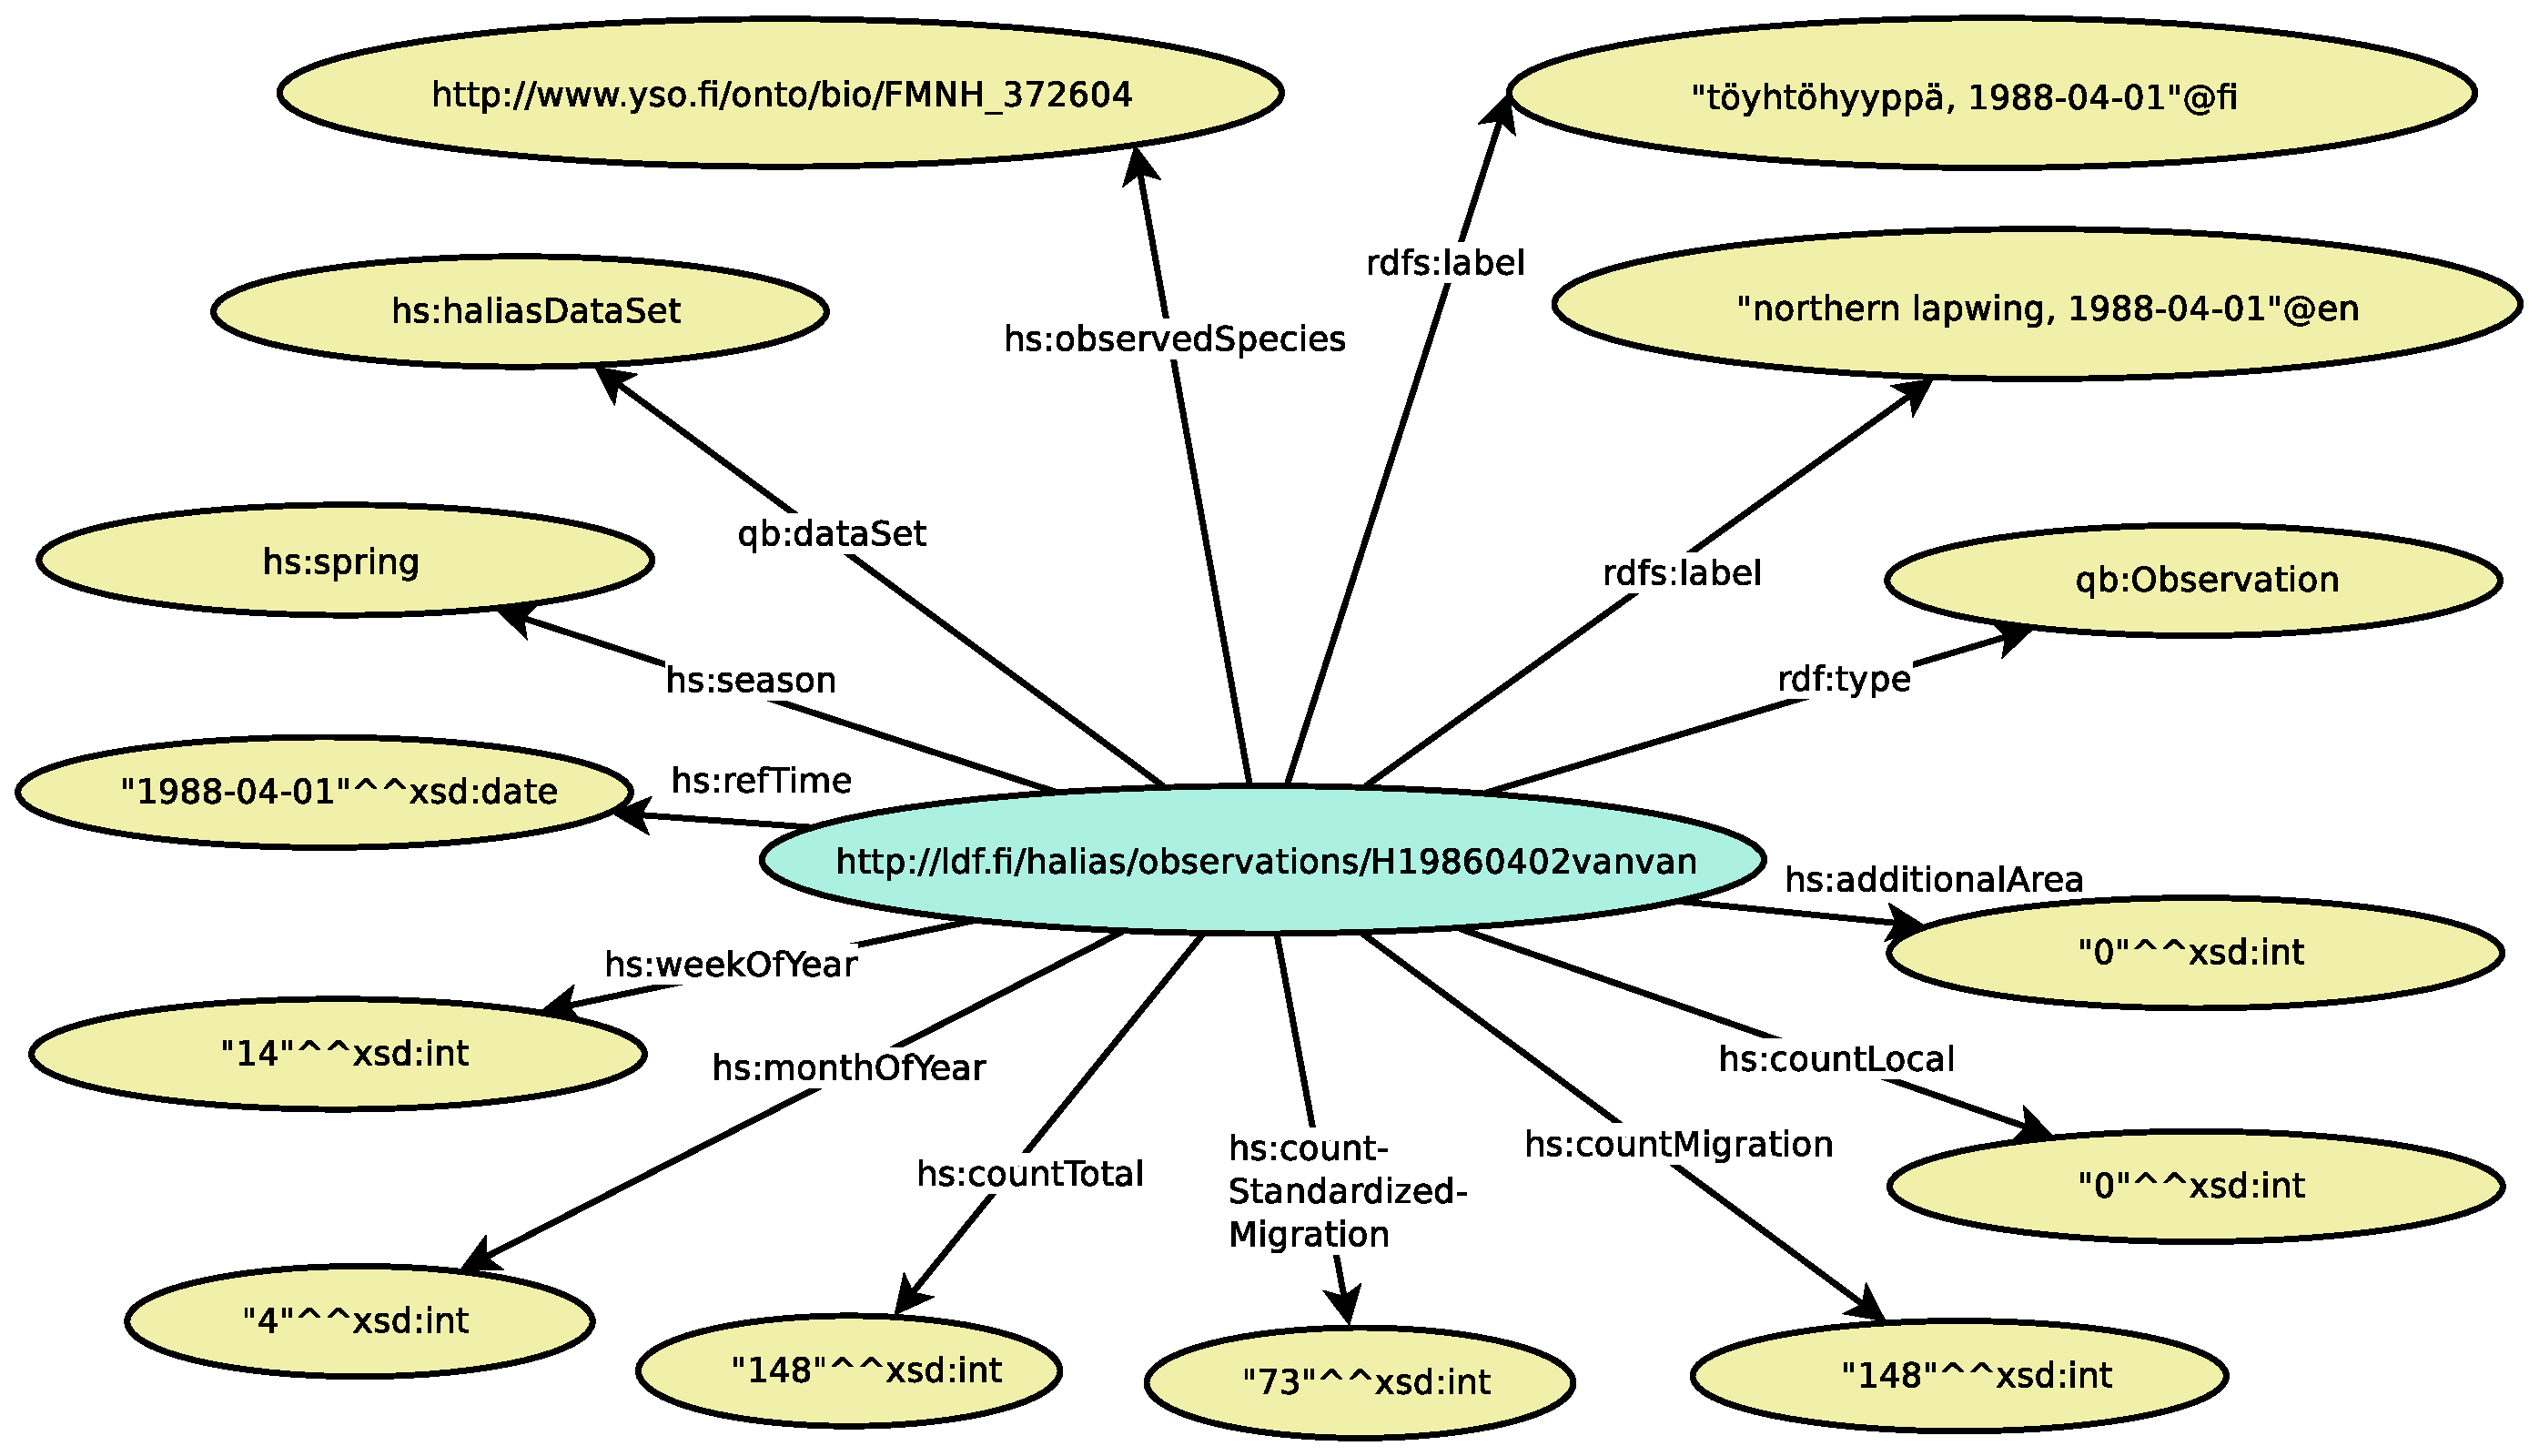
\includegraphics[clip=true, width=\textwidth]{havaintograafi}
\caption{Daily observation data of one species from one day in RDF format~\cite{koho2015gradu}.}
\label{fig: havaintograafi}
\end{figure}


%%%%%%%%%%%%%%%%%%%
\section{Methodology}
%%%%%%%%%%%%%%%%%%%

For association analysis we take a subset of the dimensions of the data cubes and transform these to market basket transactions or sequence database. In this transformation it is easy to combine bird observations, weather observations and information from the used ontologies. The transformed data is stored in \emph{JSON} or text files, which is then read in when doing analysis.

For simplicity, we first try to find interesting patterns using just the bird observations. We will do frequent pattern mining to find the most frequently observed species and species combinations, without using the daily counts. We could also use the observed counts and generate quantitative association rules, which might reveal some interesting patterns, but is probably very slow to calculate.

Next, we will try sequential pattern mining, using the timestamps already present in the data. This would probably reveal something interesting, but is again very slow to calculate.

The analysis is done using Python 3 and various modules. Plotting and examining the data was done mainly with \emph{IPython notebook}\footnote{\url{http://ipython.org/notebook.html}} and \emph{pandas} (Python Data Analysis Library)\footnote{\url{http://pandas.pydata.org/}}. Conversion from RDF uses \emph{RDFLib}\footnote{\url{https://github.com/RDFLib/rdflib}}. 

Pattern mining implementations are self-made and available online\footnote{\url{https://github.com/razz0/DataMiningProject}}. They include algorithms for finding frequent itemsets, frequent sequential patterns and rule generation. The algorithms are based on the \emph{Apriori algorithm}~\cite{tan2006introduction}.

The pattern mining algorithms are somewhat memory efficient, but are computationally slow. They only use a single CPU core for all calculations and they use standard Python data types, which are flexible, but computationally inefficient. An attempt was made to optimize an Apriori based algorithm for speed, by first profiling the algorithm at execution time and finding the bottlenecks. The pruning step seems to be clearly the most computationally intensive part of the algorithm. % TODO: Tarkasta kirjasta

We attempted to optimize the pruning by using multiple processes, running in different CPU cores, using Python module Joblib\footnote{\url{https://pythonhosted.org/joblib/}}, which provides an improved interface to Python standard library \emph{multiprocessing} module. However, the processes running in parallel cannot access shared resources in memory, leading to extensive copying of large data structures and longer execution times. This could be overcome by switching to use data structures from NumPy\footnote{\url{http://www.numpy.org/}}, which are optimized for speed and allow shared access from multiple processes.


\emph{Orange Data Mining Toolbox}\footnote{\url{http://orange.biolab.si/}} was also tried for analysis, but it wasn't able to cope with even simple market basket transaction data of all the daily observed taxa in the dataset (7419 days, 378 taxa).


%%%%%%%%%%%%%%%%%%%
\section{Analysis results}
%%%%%%%%%%%%%%%%%%%

The dataset is quite large for many association analysis tasks, which is why the focus has been on using simple methods.


\subsection{Visualization}
%%%%%%%%%%%%%%%%%%%

Visualizations of the data can easily convey important patterns in the data. \ref{fig: embhor_years}

\begin{figure}[htb]
\centering
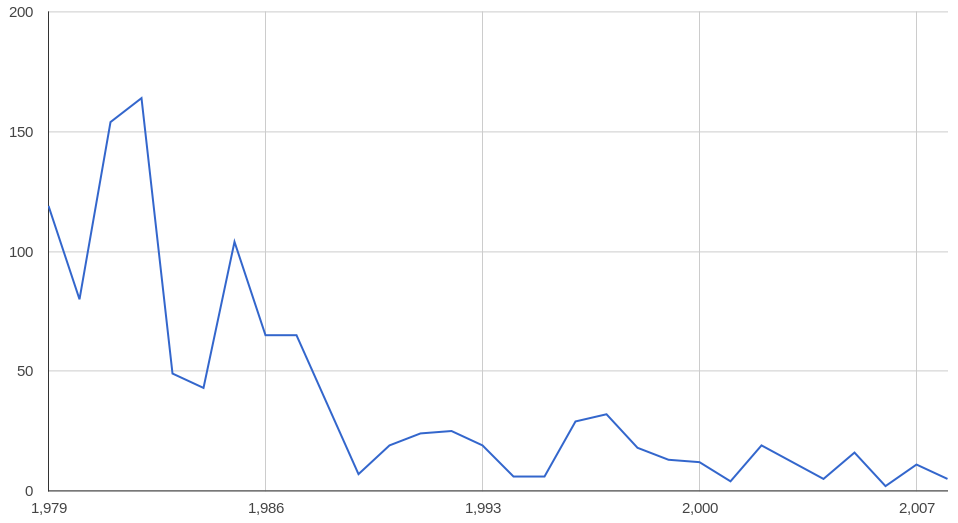
\includegraphics[clip=true, width=\textwidth]{embhor_years}
\caption{embhor years}
\label{fig: embhor_years}
\end{figure}

Foo\ref{fig: phacar_years}.

\begin{figure}[htb]
\centering
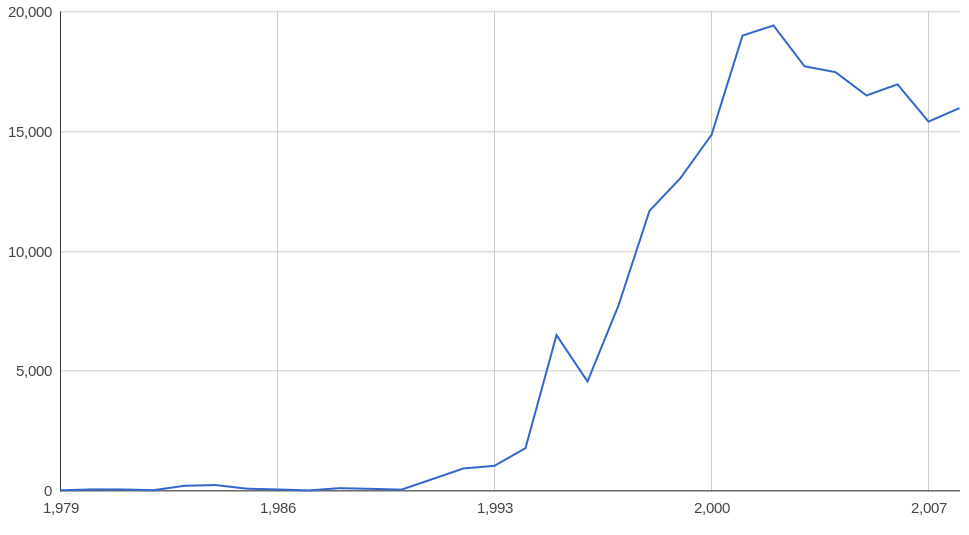
\includegraphics[clip=true, width=\textwidth]{phacar_years}
\caption{phacar years}
\label{fig: phacar_years}
\end{figure}

Bar\ref{fig: embhor_weeks}.

\begin{figure}[htb]
\centering
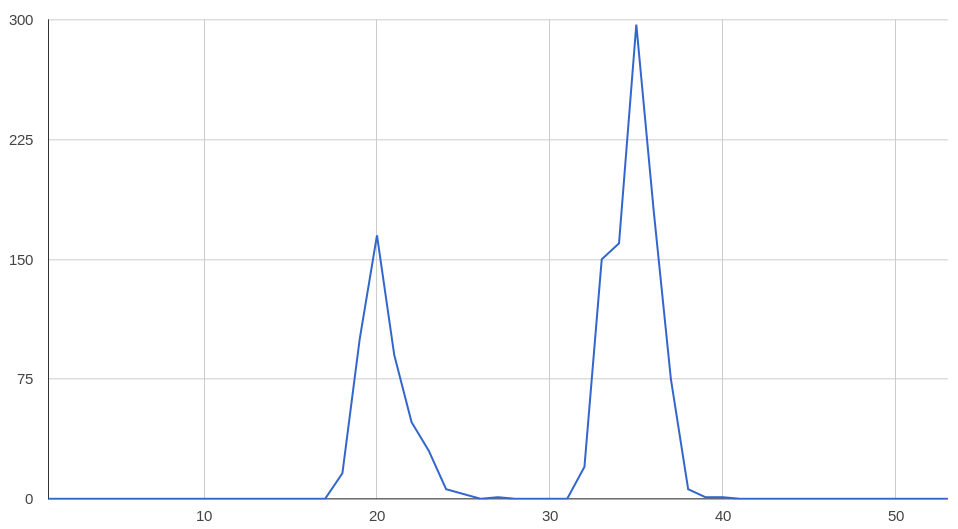
\includegraphics[clip=true, width=\textwidth]{embhor_weeks}
\caption{embhor weeks}
\label{fig: embhor_weeks}
\end{figure}

Baz\ref{fig: phacar_weeks}.

\begin{figure}[htb]
\centering
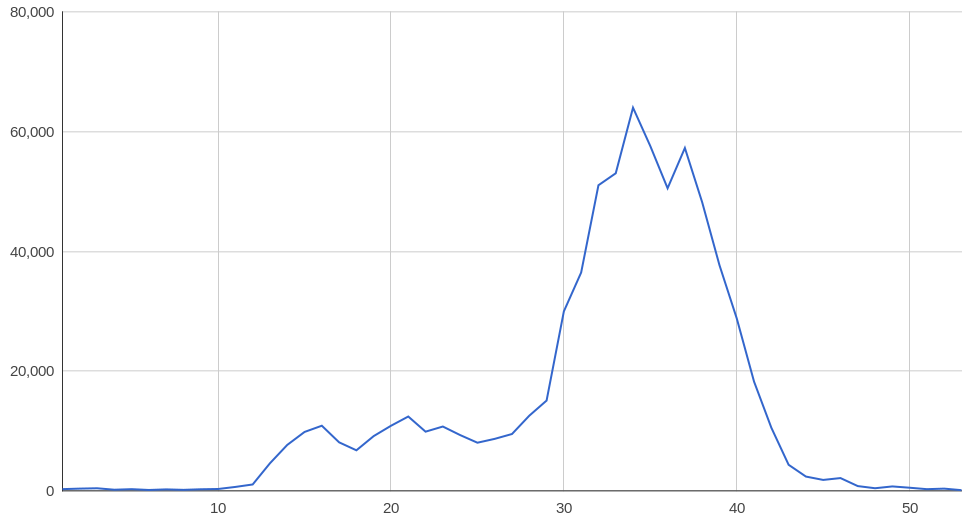
\includegraphics[clip=true, width=\textwidth]{phacar_weeks}
\caption{phacar weeks}
\label{fig: phacar_weeks}
\end{figure}


\subsection{Frequent itemsets}
%%%%%%%%%%%%%%%%%%%

Analysing daily observed species as market basket transactions, we can examine the most commonly observed species and species combinations.

The most common species is <varis, \emph{Corvus corone}, carrion crow> with support 0.951. For support $0.5$, the largest frequent itemset consists of the following species:

%\begin{itemize}
\hangindent=0.7cm
<harmaalokki, \emph{Larus argentatus}, herring gull>, \\
<isokoskelo, \emph{Mergus merganser}, goosander/common merganser>, \\
<kalalokki, \emph{Larus canus}, mew gull>, \\
<merilokki, \emph{Larus marinus}, great black-backed gull>, \\
<sinisorsa, \emph{Anas platyrhynchos}, mallard>, \\
<sinitiainen, \emph{Parus caeruleus}, blue tit>, \\
<talitiainen, \emph{Parus major}, great tit>, \\
<telkkä, \emph{Bucephala clangula}, common goldeneye>, \\
<varis, \emph{Corvus corone}, carrion crow>, \\
<viherpeippo, \emph{Carduelis chloris}, european greenfinch> \\
%\nohang
%\end{itemize}

This is the largest combination of species that is observed in half of the observation days. These species are very common and observable almost all year round. Individually all of the listed species have support over $0.75$.


%\subsection{Frequent taxon sequences}
%%%%%%%%%%%%%%%%%%%


%\subsection{Rule generation}
%%%%%%%%%%%%%%%%%%%

%By generating some high confidence rules~\cite{tan2006introduction} from frequent itemsets we can get

\subsection{Analysing species itemsets}
%%%%%%%%%%%%%%%%%%%

We created itemsets of all observed taxa, consisting of species name, its' characteristics, conservation status and commonness measure at Halias. All of this species information is already present in the taxon ontology, but here we transform the information from ontologies to a format that allows us to use common data mining algorithms. Analysing these itemsets as market basket transactions we can infer frequent rules, but these mostly tell us about the used characteristics ontology and its' annotations.
% TODO: high lift implies something contradictory?
Table \ref{fig: species_itemsets} shows two examples of a frequent generated rule with the rules' measures~\cite{tan2006introduction} for confidence, support, lift and IS measure.
The ''Late spring -- early summer'' and ''Late summer -- autumn'' are part of the characteristics ontology, describing seasonal occurence of the species in Finland.

\begin{table}[ht]
\centering
\begin{tabularx}{\textwidth}{| >{\hsize=3.2\hsize}X | >{\hsize=0.5\hsize}X | >{\hsize=0.4\hsize}X | >{\hsize=0.3\hsize}X | >{\hsize=0.6\hsize}X |}
  \hline
  \textbf{Rule} & \small \textbf{Con\-fi\-den\-ce} & \small \textbf{Sup\-port} & \small \textbf{Lift} & \small \textbf{IS measure}\\
  \hline
  \small
  \{Late spring -- early summer, beak dark, head multicoloured, iris dark, upperside atleast 2-coloured\}
  $\rightarrow$
  \{Late summer -- autumn\} 
  & 0.99 & 0.51 & 1.26 & 0.80 \\
  \hline
  \small
  \{Common species at Halias\}
  $\rightarrow$
  \{Late spring -- early summer, Late summer -- autumn\} 
  & 0.93 & 0.51 & 1.19 & 0.78 \\
  \hline
\end{tabularx}
\caption{Two examples of frequent rules generated from species itemsets.}
\label{fig: species_itemsets}
\end{table}



\subsection{Species itemsets with weather variables}

The species itemsets were further processed by leaving out all taxa that don't have characteristics annotations, and enriching the itemsets with weather averaged variables. For each species we add an average of the weather variables measured each day from sunrise to sunset and weight them with the count of birds that have been observed that day. So we get an average weather condition in which the species has been observed. All of the averaged weather variables were categorized in three categories: ''low'', ''average'' and ''high''. The categories contain respectively the lowest, middle and highest third of all numbers. The limits of the categories are shown in table \ref{fig: weather cats}.

\begin{table}[ht]
\centering
\begin{tabularx}{\textwidth}{| >{\hsize=1.0\hsize}X | >{\hsize=1.0\hsize}X | >{\hsize=1.0\hsize}X | >{\hsize=1.0\hsize}X |}
  \hline
  \textbf{Variable} & \textbf{Low} & \textbf{Average} & \textbf{High} \\
  \hline
  \textbf{Pressure} & [994.3, 1013.0] & (1013.0, 1014.5] & (1014.5, 1039.0] \\
  \textbf{Cloud cover} & [0.0, 3.9] & (3.9, 4.5] & 4.5, 8.0] \\ 
  \textbf{Humidity} & [56.0, 79.7] & (79.7, 81.8]        & (81.8, 93.7] \\
  \textbf{Rainfall} & [0.0, 1.0] & (1.0, 1.4]          & (1.4, 18.0] \\ 
  \textbf{Temperature} & [-2.4, 8.4]     & (8.4, 12.1]         & (12.1, 20.0] \\ 
  \textbf{Wind speed} & [0.1, 8.0]      & (8.0, 18.8]         & (18.8, 2109.0] \\
  \hline
\end{tabularx}
\caption{Weather variable category limits derived from averaged weather variables by dividing them into three equally sized chunks.}
\label{fig: weather cats}
\end{table}

We generated association rules from these species itemsets. Some examples of these rules with their measurements are given in table \ref{fig: species_itemsets_2_rules}.

\begin{table}[ht]
\centering
\begin{tabularx}{\textwidth}{| >{\hsize=3.2\hsize}X | >{\hsize=0.5\hsize}X | >{\hsize=0.4\hsize}X | >{\hsize=0.3\hsize}X | >{\hsize=0.6\hsize}X |}
  \hline
  \textbf{Rule} & \small \textbf{Con\-fi\-den\-ce} & \small \textbf{Sup\-port} & \small \textbf{Lift} & \small \textbf{IS measure}\\
  \hline
  \small
  \{Rare at Halias\}
  $\rightarrow$
  \{Head multicoloured, Late summer -- autumn, Upperside atleast two-coloured, Late spring -- early summer\} 
  & 0.89 & 0.30 & 0.99 & 0.55 \\
  \hline
  \small
  \{a\}
  $\rightarrow$
  \{b\} 
  & 0 & 0 & 0 & 0 \\
  \hline
\end{tabularx}
\caption{Some association rules generated from species itemsets.}
\label{fig: species_itemsets_2_rules}
\end{table}


%%%%%%%%%%%%%%%%%%%
\section{Conclusions}
%%%%%%%%%%%%%%%%%%%



%%%%%%%%%%%%%%%%%%%
\section{Discussion}
%%%%%%%%%%%%%%%%%%%




\pagebreak

% --- References ---
%
% bibtex is used to generate the bibliography. The babplain style
% will generate numeric references (e.g. [1]) appropriate for theoretical
% computer science. If you need alphanumeric references (e.g [Tur90]), use
%
% \bibliographystyle{babalpha-lf}
%
% instead.

\bibliographystyle{babalpha-lf}
\bibliography{references-en}

\lastpage

\end{document}
